\documentclass{article}
\usepackage{tikz}
\usetikzlibrary{arrows.meta}

\begin{document}

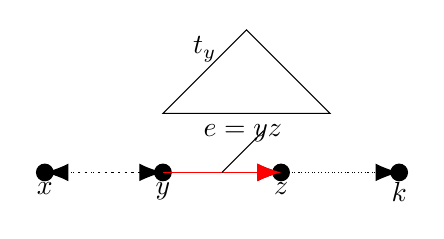
\begin{tikzpicture}[scale=1.5]
    % Define coordinates for the vertices
    \coordinate (x) at (-1,0);
    \coordinate (y) at (0,0);
    \coordinate (z) at (1,0);
    \coordinate (k) at (2,0);

    % Draw the vertices as filled circles
    \filldraw[black] (x) circle (2pt) node[below] {$x$};
    \filldraw[black] (y) circle (2pt) node[below] {$y$};
    \filldraw[black] (z) circle (2pt) node[below] {$z$};
    \filldraw[black] (k) circle (2pt) node[below] {$k$};

    % Draw the dotted directed edges forming the cycle C
    \draw[dotted,-{Latex[length=3mm]}] (x) -- (y);
    \draw[dotted,-{Latex[length=3mm]}] (y) -- (z);
    \draw[dotted,-{Latex[length=3mm]}] (z) -- (k);
    \draw[dotted,-{Latex[length=3mm]}] (k) -- (x);

    % Draw the solid edge e = yz
    \draw[-{Latex[length=3mm]},red] (y) -- (z);

    % Draw the label for the triangle t_y
    \draw (0,0.5) -- ++(45:1) node[midway,above] {$t_y$} -- ++(-45:1) -- cycle;

    % Draw the label for the edge e = yz
    \draw (0.5,0) -- ++(45:0.5) node[midway,above] {$e = yz$};
\end{tikzpicture}

\end{document}